\section{Merging Strategy and Error Analysis}\label{sec:voting}

\paragraph{Output Analysis}
% Individual Model Performance Analysis
We first analyze the individual model performance of \VIT{}, \CROP{}, and \CONV{} on the validation set.
\begin{figure}[htbp]
    \centering
    \begin{subfigure}{0.32\textwidth}
        \centering
        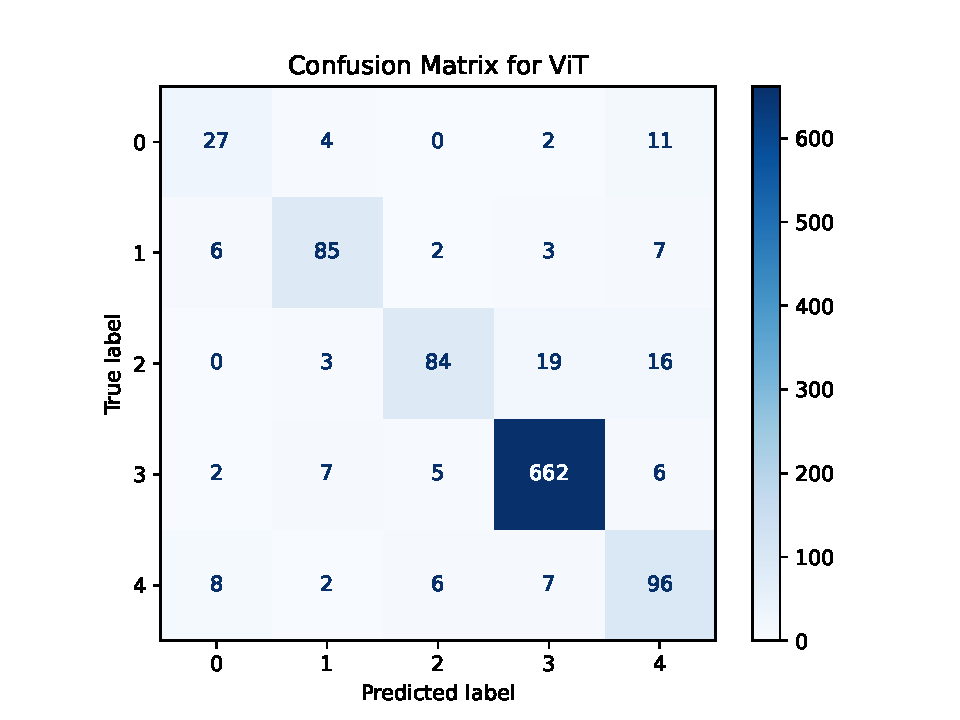
\includegraphics[width=\linewidth]{graphs/ModelMergeStudy/ViT.pdf}
        \caption{\VIT}
    \end{subfigure}
    \begin{subfigure}{0.32\textwidth}
        \centering
        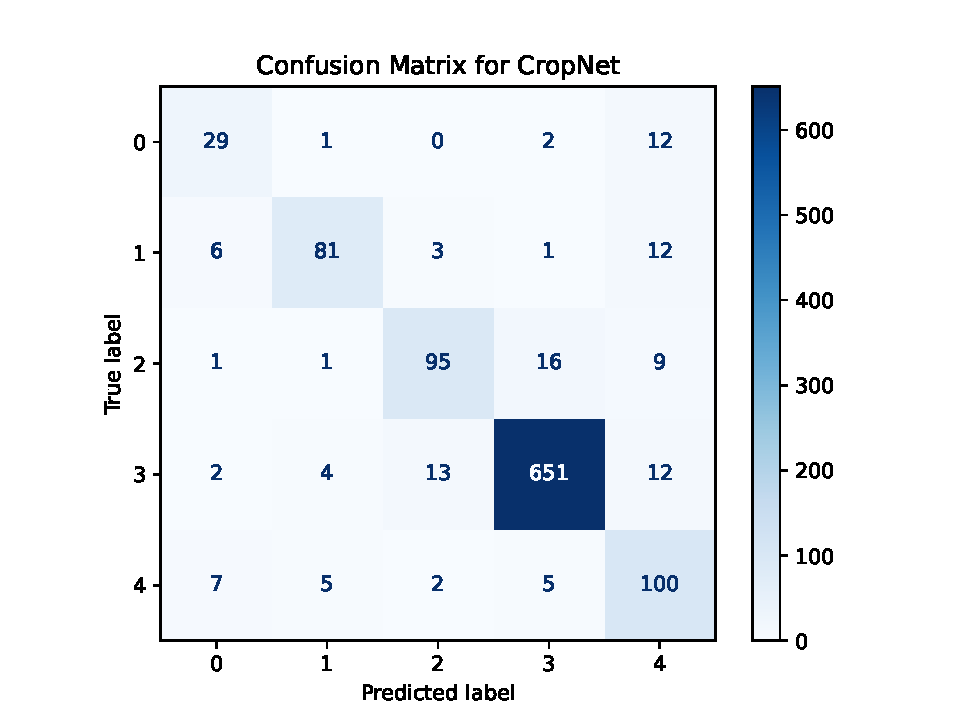
\includegraphics[width=\linewidth]{graphs/ModelMergeStudy/CropNet.pdf}
        \caption{\CROP}
    \end{subfigure}
    \begin{subfigure}{0.32\textwidth}
        \centering
        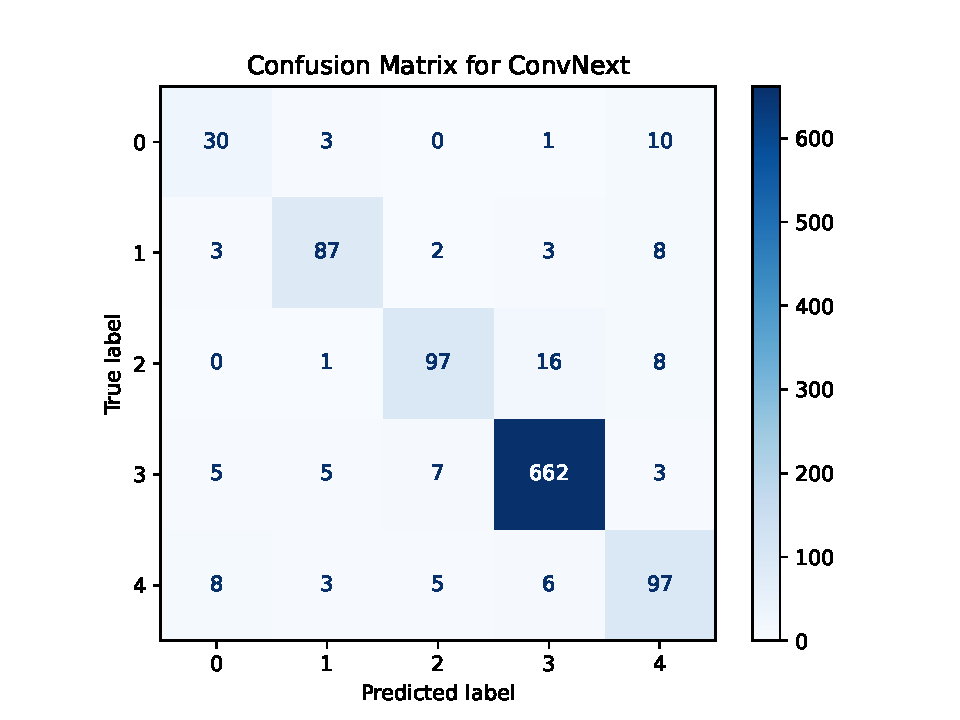
\includegraphics[width=\linewidth]{graphs/ModelMergeStudy/ConvNext.pdf}
        \caption{\CONV}
    \end{subfigure}
    \caption{Confusion Matrix for Three Models}
    \label{confusionMatrix}
\end{figure}

Fig~\ref{confusionMatrix} presents the confusion matrices for the three models: \VIT{}, \CROP{}, and \CONV{}. Each matrix illustrates how well the respective model classifies the validation dataset. The horizontal axis represents the label predicted by the model, while the vertical axis indicates the actual results. Thus, the diagonal elements indicate the correctly classified images, while the off-diagonal elements represent the misclassified instances.

The evaluation of the three models indicates that the dataset is imbalanced, with class 3 dominating the data. In addition, all models achieved their highest accuracy in class 3. Conversely, class 0 presents the greatest challenge, resulting in the lowest accuracy across all models. Among them, \CONV{} stands out for its overall accuracy, excelling in classes 0, 1, 2, and 3, though \CROP{} slightly performs better in class 4. Notably, \CROP{} and \VIT{} demonstrate complementary strengths, with \CROP{} performing better in classes 0, 2, and 4, while \VIT{} shows an advantage in classes 1 and 3. Therefore, combining these models together could yield better results.
\paragraph{Hard Voting}
Hard voting, also known as majority voting, involves each model casting a "vote" for a specific class, with the final outcome determined by the majority of votes from all models. This method does not take into account the probabilities associated with each model's prediction. As demonstrated in Algorithm \ref{alg:hardvote}, we implemented hard voting based on the three models discussed previously. In the event of a tie, we have observed that we will default to the result from \CONV{} as the final outcome.


% persudo code
\begin{algorithm}[ht]
\SetAlgoLined
\KwData{Input data $X$, Models \CONV{}, \CROP{}, \VIT{}}
\KwResult{Final prediction $y$}
\caption{Hard Voting Ensemble with Tie-Breaker}
\label{alg:hardvote}
$y_{\text{conv}} \gets$ \CONV.predict($X$)\;
$y_{\text{crop}} \gets$ \CROP.predict($X$)\;
$y_{\text{vit}} \gets$ \VIT.predict($X$)\;
$votes \gets \{y_{\text{conv}}, y_{\text{crop}}, y_{\text{vit}}\}$\;
$count \gets$ count occurrences of each class in $votes$\;
\eIf{maximum count in $count$ is unique}{
    $y \gets$ class with maximum count in $count$\;
}{
    $y \gets y_{\text{conv}}$ \tcp*{Tie-breaker: choose \CONV{} prediction}
}
\Return{$y$}
\end{algorithm}

As shown in Fig~\ref{fig: hard voting}, the hard voting algorithm allowed us to combine the strengths of each individual model, reducing wrong predictions and enhancing overall accuracy. However, hard voting could also lead to suboptimal results when models vary significantly in accuracy. For example, if a model is indecisive between two classes, using its hard vote may lead to an inaccurate result.

\paragraph{Soft Voting}

In contrast, soft voting addresses this issue by calculating the probability scores from each model's predictions. As illustrated in Fig~\ref{fig:cdf}, we compared the probability differences in cumulative distribution between the ground truth and predicted variables. The results indicate that approximately $20\%$ shows no significant difference, while $40\%$ shows only minor differences. This suggests that soft voting could also yield favorable results.

We implemented a soft voting algorithm as shown in Algorithm~\ref{soft voting}. Each model predicts a corresponding probability for each class. Then, we sum these probabilities to calculate an overall probability. Finally, we select the class with the highest overall probability as the final predicted result.

\begin{figure}
    \centering
    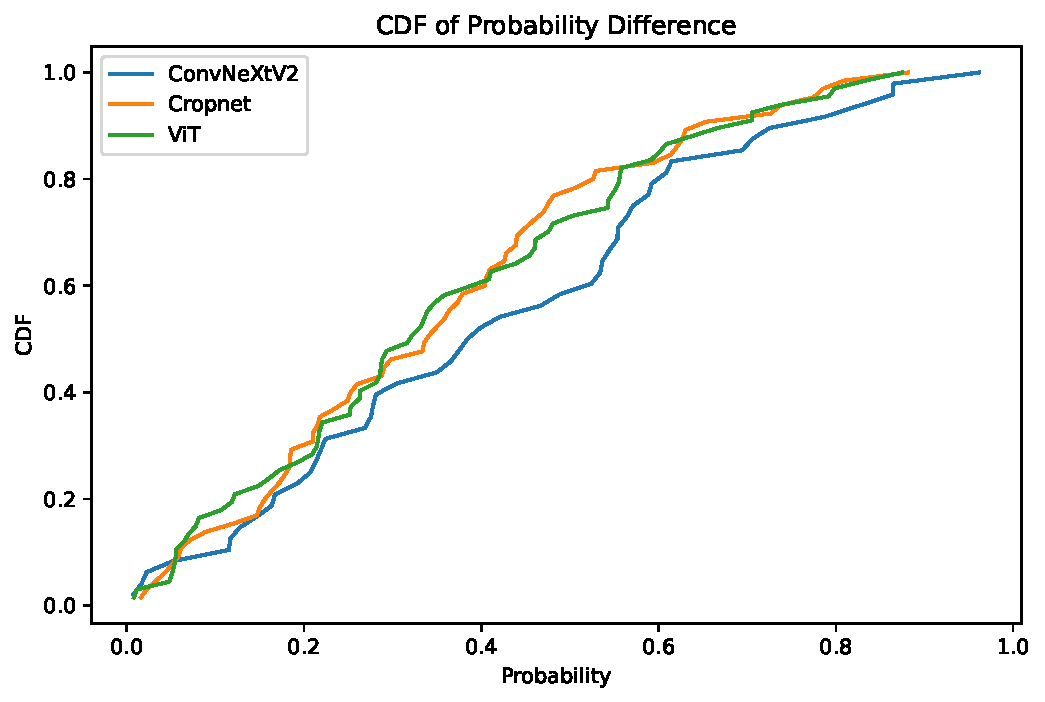
\includegraphics[width=0.7\linewidth]{graphs/ModelMergeStudy/cdf}
    \caption{CDF for Probability Difference}
    \label{fig:cdf}
\end{figure}

\begin{algorithm}[ht]
\SetAlgoLined
\KwData{Input data $X$, Models \CONV{}, \CROP{}, \VIT{} with probability outputs}
\KwResult{Final prediction $y$}
\caption{Soft Voting Ensemble}
\label{soft voting}
$P_{\text{conv}} \gets$ ConvNet.predict\_proba($X$) \tcp*{Probability output of ConvNet}
$P_{\text{crop}} \gets$ CropNet.predict\_proba($X$) \tcp*{Probability output of CropNet}
$P_{\text{vit}} \gets$ ViT.predict\_proba($X$) \tcp*{Probability output of ViT}
$P_{\text{total}} \gets P_{\text{conv}} + P_{\text{crop}} + P_{\text{vit}}$
$y \gets \arg\max(P_{\text{total}})$ \tcp*{Select class with highest summed probability}

\Return{$y$}

\end{algorithm}

\paragraph{Conclusion}

\begin{figure}[t]
    \centering
    \begin{subfigure}{0.45\textwidth}
        \centering
        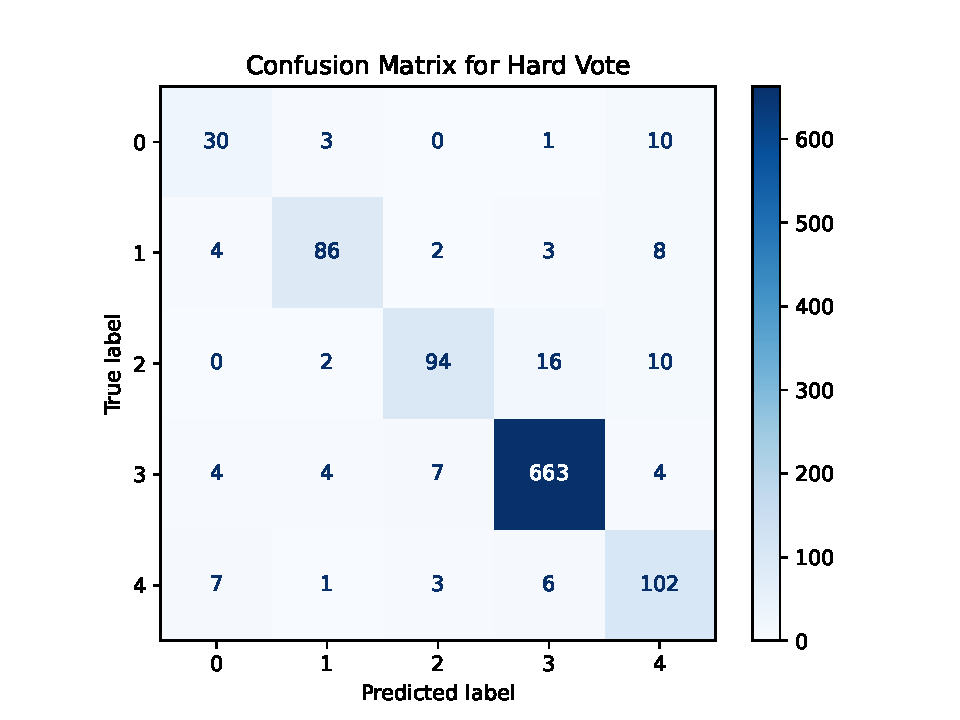
\includegraphics[width=\linewidth]{graphs/ModelMergeStudy/Hard Vote.pdf}
        \caption{Hard Voting}
        \label{fig: hard voting}
    \end{subfigure}
    \begin{subfigure}{0.45\textwidth}
        \centering
        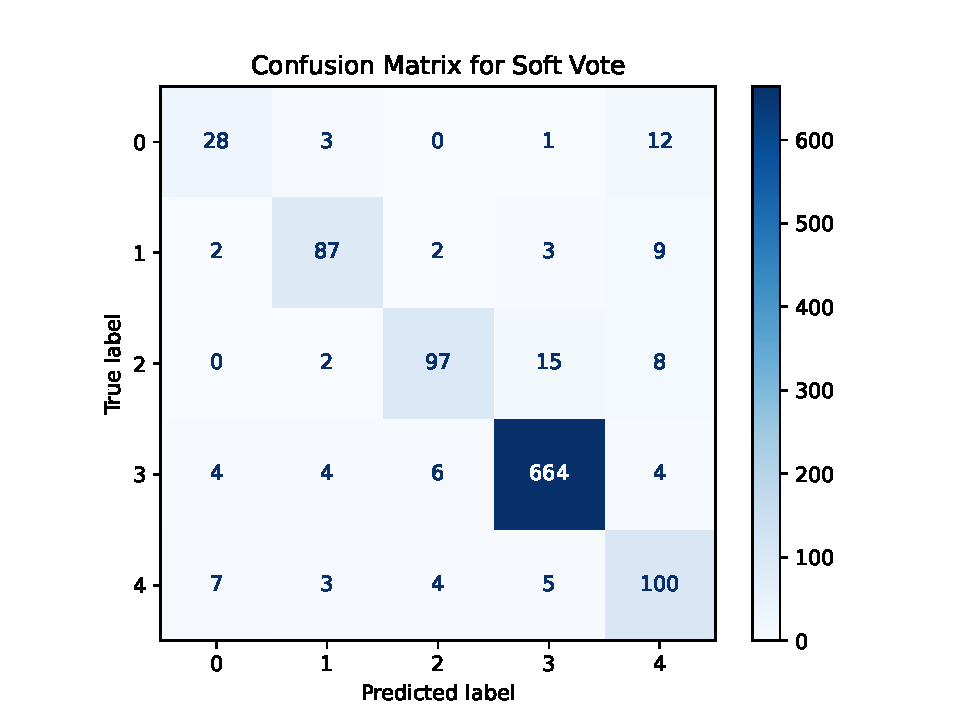
\includegraphics[width=\linewidth]{graphs/ModelMergeStudy/Soft Vote.pdf}
        \caption{Soft Voting}
        \label{fig: soft voting}
    \end{subfigure}
    \caption{Confusion Matrix for Hard Voting and Soft Voting}
    \label{hard soft confusionMatrix}
\end{figure}

Fig~\ref{hard soft confusionMatrix} shows the confusion matrix for both hard and soft voting. Both algorithms share the common advantage of effectively improving overall accuracy. However, there are slight differences in performance across specific classes. Compared to soft voting, hard voting yields more accurate predictions for classes 0 and 4 but performs less effectively for classes 1, 2, and 3. Overall, soft voting achieves a higher accuracy rate.

Compared to hard voting, soft voting benefits from the use of more granular probability scores, which reduces sensitivity to wrong predictions, better handles class imbalances in the original data, and offers improved generalization ability. Therefore, we have decided to use soft voting as our chosen method.

Our soft voting method reached $90.79\%$ (rank 17/3901) in the public benchmark.

\section{Further Improvement in The Merging Process}

Besides Hard Voting and Soft Voting discussed in Section \ref{sec:voting}, we proposed a voting method called \textit{Soft Voting with Confidence}. The general idea is that if a model generates more extreme probabilities, it should be more confident, and we should assign it greater voting weight. Conversely, if the model's results are ambiguous, we should reduce its weight.

We define a \textbf{confidence} $c(p)$ as a function
\begin{equation}
    c: [0, 1] \to [0,\infty)
\end{equation}
with the following properties:
\begin{enumerate}
    \item $c(0) = c(1) = 1$;\label{prop:eq1}
    \item $c$ is continuous in $[0, 1]$;\label{prop:cont}
    \item $c$ is a quasiconvex function, which means:\begin{equation}
        \forall x_1, x_2, t\in [0, 1]^3, c(tx_1 + (1-t)x_2)\le \max\{c(x_1), c(x_2)\}
    \end{equation}\label{prop:convex}
\end{enumerate}
Property~\ref{prop:eq1} suggests that if the model predicts probability $0$ or $1$, it should have full confidence. Property~\ref{prop:cont} ensures a slight change in prediction won't affect too much. Property~\ref{prop:convex} defines the shape of the confidence function.

We define the voting weight
\begin{equation}
w(p) = p\cdot c(p)
\end{equation}

So the final value is
\begin{equation}
    v_{\text{total}}(i) = \sum_{m\in\text{models}}w(p_m(i))\cdot p_m(i) = \sum_{m\in\text{models}}\left(p_m(i)\right)^2\cdot c(p_m(i))
\end{equation}

We selected confidence functions
\begin{equation}
    c(p) = \frac{\cosh(2p-1)}{\cosh(0)} = \frac{e^{2p-1}+e^{-2p+1}}{e +e^{-1}}
\end{equation}
in our model.
